\documentclass[12pt]{article}
\usepackage[paperwidth=420mm,paperheight=190mm,margin=12mm]{geometry}
\usepackage[T1]{fontenc}\usepackage{lmodern,graphicx,xcolor}
\definecolor{tumblue}{RGB}{0,101,189}
\pagestyle{empty}\setlength{\parindent}{0pt}
\begin{document}
\noindent\begin{minipage}[t]{.60\textwidth}\vspace{0pt}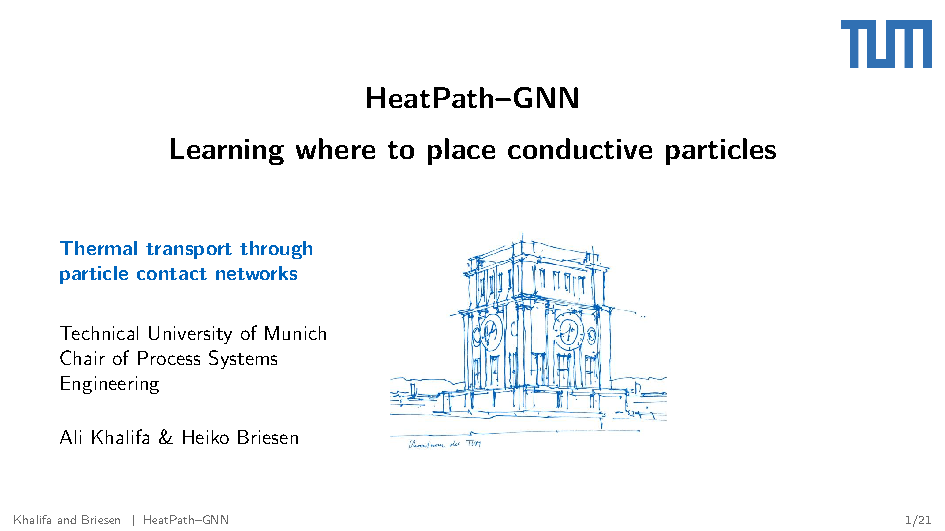
\includegraphics[page=1,width=\linewidth]{heatpath_gnn.pdf}\end{minipage}\hfill\begin{minipage}[t]{.36\textwidth}\vspace{0pt}{\Large\color{tumblue}\bfseries Slide 1}\par\vspace{.5cm}{\large HeatPath--GNN}\par\vspace{.5cm}Today I will explain a particle-allocation problem. We have a fixed packed bed and a limited amount of highly conductive material. The question is where to place that material to improve heat transfer. We first solve and optimize a physical thermal network, then train a graph neural network to propose allocations for another packing. The results cover thirty independent realizations of one packing specification.\end{minipage}\newpage
\noindent\begin{minipage}[t]{.60\textwidth}\vspace{0pt}\includegraphics[page=2,width=\linewidth]{heatpath_gnn.pdf}\end{minipage}\hfill\begin{minipage}[t]{.36\textwidth}\vspace{0pt}{\Large\color{tumblue}\bfseries Slide 2}\par\vspace{.5cm}{\large Motivation: conductive material is a limited resource}\par\vspace{.5cm}The motivation is to improve transport without increasing the conductive-material budget. An effective conductivity describes the whole bed, but it hides the individual contacts through which heat moves. The design variable here is the assignment of material to particles. We keep the geometry fixed while comparing assignments, so any difference between methods is attributable to allocation within this model. Practical manufacturing of a prescribed assignment remains a separate question.\end{minipage}\newpage
\noindent\begin{minipage}[t]{.60\textwidth}\vspace{0pt}\includegraphics[page=3,width=\linewidth]{heatpath_gnn.pdf}\end{minipage}\hfill\begin{minipage}[t]{.36\textwidth}\vspace{0pt}{\Large\color{tumblue}\bfseries Slide 3}\par\vspace{.5cm}{\large The allocation problem}\par\vspace{.5cm}This schematic illustrates the hypothesis, not a measured packing or an optimal solution. Both arrangements contain the same number of orange particles. Connecting conductive particles could reduce resistance, but the whole network, including interfaces with low-conductivity particles, determines the result. The actual problem has five hundred particles and three size classes. We enforce the budget separately within each class, which also fixes the high-conductivity solid volume.\end{minipage}\newpage
\noindent\begin{minipage}[t]{.60\textwidth}\vspace{0pt}\includegraphics[page=4,width=\linewidth]{heatpath_gnn.pdf}\end{minipage}\hfill\begin{minipage}[t]{.36\textwidth}\vspace{0pt}{\Large\color{tumblue}\bfseries Slide 4}\par\vspace{.5cm}{\large Thirty packings with the same nominal porosity}\par\vspace{.5cm}Each realization contains the same exact size distribution and occupies the same fixed-volume cell. Nominal porosity is calculated from the sum of sphere volumes divided by cell volume. With overlapping DEM spheres, this nominal quantity is not exactly the geometrical void fraction of their union. The modulus is deliberately softened. The final packings pass the particle-count, diameter, porosity, kinetic-energy and wall-spanning checks. We vary the random initialization, not the physical specification.\end{minipage}\newpage
\noindent\begin{minipage}[t]{.60\textwidth}\vspace{0pt}\includegraphics[page=5,width=\linewidth]{heatpath_gnn.pdf}\end{minipage}\hfill\begin{minipage}[t]{.36\textwidth}\vspace{0pt}{\Large\color{tumblue}\bfseries Slide 5}\par\vspace{.5cm}{\large A contact network represents steady heat conduction}\par\vspace{.5cm}Each particle is represented by one temperature. For every contact, the heat leaving one particle enters its neighbour with the opposite sign. Summing the nodal balances therefore cancels internal heat exchanges. The boundary heat rate defines the effective conductivity. Hot and cold wall temperatures are 301 and 300 kelvin. This is a steady contact-conduction model. It excludes fluid-gap conduction, radiation and convection, and it does not resolve temperature variations inside each particle.\end{minipage}\newpage
\noindent\begin{minipage}[t]{.60\textwidth}\vspace{0pt}\includegraphics[page=6,width=\linewidth]{heatpath_gnn.pdf}\end{minipage}\hfill\begin{minipage}[t]{.36\textwidth}\vspace{0pt}{\Large\color{tumblue}\bfseries Slide 6}\par\vspace{.5cm}{\large Thermal conductance follows contact size and material}\par\vspace{.5cm}The contact radius comes from the Hertz geometrical relation between overlap and effective radius. The thermal model then adds two half-space spreading resistances, each equal to one over four k a. For identical conductivities this gives G equals two k a. An isothermal wall has zero spreading resistance on its side, leaving four k a. The corrected prefactor is used throughout this campaign. The formulas are idealizations, especially when the contact radius is not small compared with the particle radius.\end{minipage}\newpage
\noindent\begin{minipage}[t]{.60\textwidth}\vspace{0pt}\includegraphics[page=7,width=\linewidth]{heatpath_gnn.pdf}\end{minipage}\hfill\begin{minipage}[t]{.36\textwidth}\vspace{0pt}{\Large\color{tumblue}\bfseries Slide 7}\par\vspace{.5cm}{\large Every method uses the same conductive-material budget}\par\vspace{.5cm}The optimization is discrete: a particle is assigned either low or high conductivity. The constraints are exact within each size class, not just over the total count. Because all particles within a class share their diameter, fixing those counts also fixes the conductive-material volume. We do not alter positions, radii or contact topology when comparing allocations on a packing. This isolates the value of arranging the material intelligently.\end{minipage}\newpage
\noindent\begin{minipage}[t]{.60\textwidth}\vspace{0pt}\includegraphics[page=8,width=\linewidth]{heatpath_gnn.pdf}\end{minipage}\hfill\begin{minipage}[t]{.36\textwidth}\vspace{0pt}{\Large\color{tumblue}\bfseries Slide 8}\par\vspace{.5cm}{\large Reference allocations and the search teacher}\par\vspace{.5cm}Random allocation provides a distribution rather than a single lucky or unlucky baseline. Degree asks whether local connectivity alone is enough. Heat-path ranking first solves a homogeneous thermal network, then prioritizes particles carrying more heat. The search evaluates same-size swaps to preserve the quotas. Its result is a strong reference obtained with a fixed computational budget. We have not proved global optimality, so I will call it best-found search rather than the optimum.\end{minipage}\newpage
\noindent\begin{minipage}[t]{.60\textwidth}\vspace{0pt}\includegraphics[page=9,width=\linewidth]{heatpath_gnn.pdf}\end{minipage}\hfill\begin{minipage}[t]{.36\textwidth}\vspace{0pt}{\Large\color{tumblue}\bfseries Slide 9}\par\vspace{.5cm}{\large Training and later use have different workflows}\par\vspace{.5cm}Training is expensive because we solve many candidate allocations on each training packing. Those results provide supervision. Later use requires a new geometry, one homogeneous baseline solve for physical input features, a GNN evaluation, exact within-size selection and a final thermal solve. Therefore GNN scoring time alone is not total design time. In the present study, later use is emulated by withholding one packing at a time.\end{minipage}\newpage
\noindent\begin{minipage}[t]{.60\textwidth}\vspace{0pt}\includegraphics[page=10,width=\linewidth]{heatpath_gnn.pdf}\end{minipage}\hfill\begin{minipage}[t]{.36\textwidth}\vspace{0pt}{\Large\color{tumblue}\bfseries Slide 10}\par\vspace{.5cm}{\large The GNN combines local geometry with baseline physics}\par\vspace{.5cm}The network is not asked to infer everything from geometry. A homogeneous thermal solve provides temperature and heat-throughput information that is available before assigning high-conductivity particles. The edges describe contact size, orientation and baseline heat flow. The GNN exchanges information along those edges over three layers. The MLP comparison uses the same node features, which helps isolate the contribution of neighbour information, though the GNN additionally uses the edge features. Feature scalers are fit on the training packings only.\end{minipage}\newpage
\noindent\begin{minipage}[t]{.60\textwidth}\vspace{0pt}\includegraphics[page=11,width=\linewidth]{heatpath_gnn.pdf}\end{minipage}\hfill\begin{minipage}[t]{.36\textwidth}\vspace{0pt}{\Large\color{tumblue}\bfseries Slide 11}\par\vspace{.5cm}{\large Scores become a feasible allocation}\par\vspace{.5cm}The target describes how often a particle is selected across teacher allocations. We optimize a within-class listwise ranking loss, plus binary cross entropy with weight 0.2. The model produces scores, not material conductivities or guaranteed feasible assignments. We rank within each class and select the prescribed number. Three independently trained repeats are combined through their ranks. This produces exact quotas without post-hoc changes to the material budget.\end{minipage}\newpage
\noindent\begin{minipage}[t]{.60\textwidth}\vspace{0pt}\includegraphics[page=12,width=\linewidth]{heatpath_gnn.pdf}\end{minipage}\hfill\begin{minipage}[t]{.36\textwidth}\vspace{0pt}{\Large\color{tumblue}\bfseries Slide 12}\par\vspace{.5cm}{\large Each test packing is withheld from model fitting}\par\vspace{.5cm}The independent unit is the packing, not an individual particle. Splitting particles from the same bed between training and testing would expose almost the same structure on both sides. Here we hold out a whole packing, use another for validation and fit on the remaining twenty-eight. We repeat the process thirty times. These folds share training data, so they are not independent training experiments. This does not establish transfer to a new porosity, particle-size distribution, system size or material contrast.\end{minipage}\newpage
\noindent\begin{minipage}[t]{.60\textwidth}\vspace{0pt}\includegraphics[page=13,width=\linewidth]{heatpath_gnn.pdf}\end{minipage}\hfill\begin{minipage}[t]{.36\textwidth}\vspace{0pt}{\Large\color{tumblue}\bfseries Slide 13}\par\vspace{.5cm}{\large Gain and recovery answer different questions}\par\vspace{.5cm}Gain normalizes the change by the random-allocation conductivity. Recovery instead divides by the available improvement found by the search. For example, a model that improves conductivity by thirty percent when search improves it by about fifty-two percent recovers roughly fifty-eight percent of the gain. The reported values are averages of per-packing ratios, so dividing displayed ensemble means will not necessarily reproduce them exactly. R-squared is not the performance measure for this discrete allocation task.\end{minipage}\newpage
\noindent\begin{minipage}[t]{.60\textwidth}\vspace{0pt}\includegraphics[page=14,width=\linewidth]{heatpath_gnn.pdf}\end{minipage}\hfill\begin{minipage}[t]{.36\textwidth}\vspace{0pt}{\Large\color{tumblue}\bfseries Slide 14}\par\vspace{.5cm}{\large GNN improves conductivity by 30\% over random}\par\vspace{.5cm}The degree rule adds almost no average benefit. A homogeneous heat-throughput ranking is better, but both learned methods improve on it. The GNN delivers thirty percent mean gain relative to random assignment. Search still achieves substantially more, at fifty-one point eight percent. Each point is a packing, and the black summary marks show the mean and sample standard deviation. These results support learning useful allocation structure while also showing room for improvement.\end{minipage}\newpage
\noindent\begin{minipage}[t]{.60\textwidth}\vspace{0pt}\includegraphics[page=15,width=\linewidth]{heatpath_gnn.pdf}\end{minipage}\hfill\begin{minipage}[t]{.36\textwidth}\vspace{0pt}{\Large\color{tumblue}\bfseries Slide 15}\par\vspace{.5cm}{\large Absolute conductivity remains below the search reference}\par\vspace{.5cm}This slide gives the absolute scale of the conductivity changes. The mean rises from approximately 0.228 watts per metre kelvin for random assignment to 0.297 for the GNN. Search reaches approximately 0.347. The thin connecting lines preserve pairing across methods. These absolute numbers belong to the corrected contact-only model and should not be mixed with values from the earlier manuscript, which used a different thermal prefactor and packing-generation implementation.\end{minipage}\newpage
\noindent\begin{minipage}[t]{.60\textwidth}\vspace{0pt}\includegraphics[page=16,width=\linewidth]{heatpath_gnn.pdf}\end{minipage}\hfill\begin{minipage}[t]{.36\textwidth}\vspace{0pt}{\Large\color{tumblue}\bfseries Slide 16}\par\vspace{.5cm}{\large GNN beats MLP on 29 of 30 held-out packings}\par\vspace{.5cm}The GNN outperforms the MLP on twenty-nine of the thirty withheld packings. Its mean recovery is fifty-eight percent, with a standard deviation of nine point eight percentage points. This is descriptive evidence across our realizations, not a claim of independent folds or universal superiority. The gap to the search reference is still substantial. Both successful and less successful packings are included in this plot.\end{minipage}\newpage
\noindent\begin{minipage}[t]{.60\textwidth}\vspace{0pt}\includegraphics[page=17,width=\linewidth]{heatpath_gnn.pdf}\end{minipage}\hfill\begin{minipage}[t]{.36\textwidth}\vspace{0pt}{\Large\color{tumblue}\bfseries Slide 17}\par\vspace{.5cm}{\large Contact-network diagnostics help interpret allocation}\par\vspace{.5cm}The first diagnostic measures what fraction of summed absolute particle-contact heat rates occurs on contacts whose endpoints are both high-conductivity particles. This is not the fraction of net wall heat because heat can traverse multiple contacts. The second diagnostic asks whether the high-conductivity subgraph alone spans the two thermal boundaries. Low-conductivity particles can still participate in useful paths, so a spanning high-only cluster is not required for heat transfer. The random visualization uses the sampled assignment closest to the random mean.\end{minipage}\newpage
\noindent\begin{minipage}[t]{.60\textwidth}\vspace{0pt}\includegraphics[page=18,width=\linewidth]{heatpath_gnn.pdf}\end{minipage}\hfill\begin{minipage}[t]{.36\textwidth}\vspace{0pt}{\Large\color{tumblue}\bfseries Slide 18}\par\vspace{.5cm}{\large Numerical checks pass, but contact sizes need scrutiny}\par\vspace{.5cm}The conservation and mechanical acceptance checks pass. However, numerical convergence does not establish physical validity. The contact-radius ratio has a median of about 0.19 and reaches about 0.35. Those contacts are not uniformly small relative to the particles. The half-space constriction approximation and the softened mechanical generation therefore deserve further assessment. This pooled histogram is a geometry diagnostic; individual contacts from the same bed are correlated.\end{minipage}\newpage
\noindent\begin{minipage}[t]{.60\textwidth}\vspace{0pt}\includegraphics[page=19,width=\linewidth]{heatpath_gnn.pdf}\end{minipage}\hfill\begin{minipage}[t]{.36\textwidth}\vspace{0pt}{\Large\color{tumblue}\bfseries Slide 19}\par\vspace{.5cm}{\large The numerical overlap floor has little influence}\par\vspace{.5cm}A small overlap floor regularizes contact-radius evaluation. We repeat the thermal evaluation with different floor values while keeping the material assignments fixed. The largest absolute relative change is less than one thousandth of a percent. That is reassuring about this numerical choice. It does not resolve the physical contact-size concern on the previous slide, because we did not regenerate the beds under another modulus, pressure or contact model.\end{minipage}\newpage
\noindent\begin{minipage}[t]{.60\textwidth}\vspace{0pt}\includegraphics[page=20,width=\linewidth]{heatpath_gnn.pdf}\end{minipage}\hfill\begin{minipage}[t]{.36\textwidth}\vspace{0pt}{\Large\color{tumblue}\bfseries Slide 20}\par\vspace{.5cm}{\large Fast scoring still requires two thermal solves}\par\vspace{.5cm}The repeated search requires nearly fifteen thousand thermal solves per packing. GNN scoring itself is fast, averaging about eight point six milliseconds for the ensemble. But that timing excludes the baseline and final verification solves, and it does not represent total execution time. Training and teacher-data generation are additional upfront costs. A fair future timing study should include feature construction and both solves, and should report how many later allocations are needed to amortize training.\end{minipage}\newpage
\noindent\begin{minipage}[t]{.60\textwidth}\vspace{0pt}\includegraphics[page=21,width=\linewidth]{heatpath_gnn.pdf}\end{minipage}\hfill\begin{minipage}[t]{.36\textwidth}\vspace{0pt}{\Large\color{tumblue}\bfseries Slide 21}\par\vspace{.5cm}{\large Conclusions and next research steps}\par\vspace{.5cm}The main contribution is a constrained allocation workflow that combines a physical contact network with graph learning. Thirty independent packings give a clearer assessment than the earlier ten-case study. The results are promising, but the physical modelling assumptions and the remaining search-performance gap should shape the next work. A practical next algorithmic test is to initialize a short swap search with the GNN selection and compare its gain per thermal solve against random initialization. Physical sensitivity and external transfer should be evaluated before making broader claims.\end{minipage}\newpage
\end{document}
